\chapter{Evaluation and results}

    \section{Benchmarking}
        \label{sec_benchmark}

        Benchmarking a file system involves many aspects and different authors
        have done it in varying ways over the years. \citeauthor{FFS} measures
        raw throughput of data while \citeauthor{LFS} recorgnise both small
        reads and writes as well as long sustained accesses.  On the other
        hand, \citeauthor{soft_updates} looks at speed of metadata access and
        modificaiton and \citeauthor{ext4_space_maps} uses a small file
        benchmark that simulates an email server. Finally, Google use a hybrid
        approach where they try a large variety of real world representative
        data with a large distribution of sizes. In the mean time popular
        consumer review sources add random accesses of varying sizes to the mix
        \cite{servethehome_review}, input/output operations per second (IOPS)
        \cite{tomshardware_review} and many other ways of looking at
        performance of drives. These last methods are a bit different in that
        they measure drive performance without usually varying the filesystem
        (or bypassing it altogether) but they are still show representative
        results as they aim to find bottlenecks of drives and quanitfy the
        highest possible performance of likely use cases.

        Despite the variety of test methodologies two important metrics stand
        out: raw throughput and the number of individual requests they can
        fulfill. However, each must be measured under varying conditions as
        unconspicuous factor may affect performance. Things like sequentially
        reading a large file may perform like a random access because its
        contents are stored in a chain of blocks like fat32 \cite{fat32}.
        Alternatively, random file accesses may be performant while metadata
        are not due to a poor choice of data strctures in the directory
        representation for example. Even though metadata benchmarks are pure
        throughput tests they focus on the data structure implementation as an
        indicator of filesystem quality.

        To account for these quirks the devised test includes measures of pure
        workloads as well as varieties of them to represent the likely tasks
        for home or office use (\ref{sec_problem}). These include the usual
        large sequentail reads and writes as well as small and random accesses
        to get a baseline. Then a very large access to control for things like
        caches that might be speeding things up. Finally, a metadata access of
        relatively small scale file creation and deletion to simulate a home
        user searching for a filename for example. We do not test for very
        large directoies as those are likley to be rare in our use case
        \cite{contents_study}.

        % might be good without these
        % sequentail performance - very important but mostly bragging rights - most accesses are smaller
        % random - realistic but over empahsised - say it's unlikey except in search
        % metadata - likely to indicate search

        To measure these a utility written by the author of the new Linux
        system call interface io\_uring, \citeauthor{IO_uring}, is used - fio
        \cite{fio}. A fio workload is devised to benchmark the highlighted
        points above: random accesses, sequential accesses and metadata
        modificaiton. This is implemented as 8 'jobs' - individual tasks that
        fio completes. There are small (4KiB size) and large (1MiB) verisons
        of each a read, a write and a combined test. Then a sequential
        read-read combo test of 1GB of data and finally creating and removing
        100 files in a loop. Each of these tests is perfomerd in sequence for
        20 seconds each.

		% possibly citations here?
        All tests are perfomerd using the same hardware and sofware setup: a
        loopback device is set up using a regular file on the filesystem as a
        backing store. The drive is a "SAMSUNG MZVLB1T0HBLR-000L7" high speed
        NVMe drive tested on an AMD Ryzen 7 PRO 4750U CPU. The test was ran 3
        times and average values were taken. As controls two more filesystems
        were tested: ext4 (\ref{sec_ext4}) and ntfs (with the ntfs-3g driver).
        They represent the modern defauls on two of the most popular operating
        systems used today and are the most likely candidates for a user to
        compare against. For concsistency, all tests were performed by
        completely wiping each drive before commencing the benchmark.


    \section{Test results}

        The results of this benchmark are in figure \ref{fig_benchmark}.
        Combined read and write tests have the read and write components added
        toghether in the summary. The raw output for the graph can be found in
        appendinx \ref{app_benchmark}.

        % \begin{wrapfigure}{L}{0.2\textwidth}
        % \end{wrapfigure}
        \begin{figure}[h!]
            \caption{Benchmark results}
            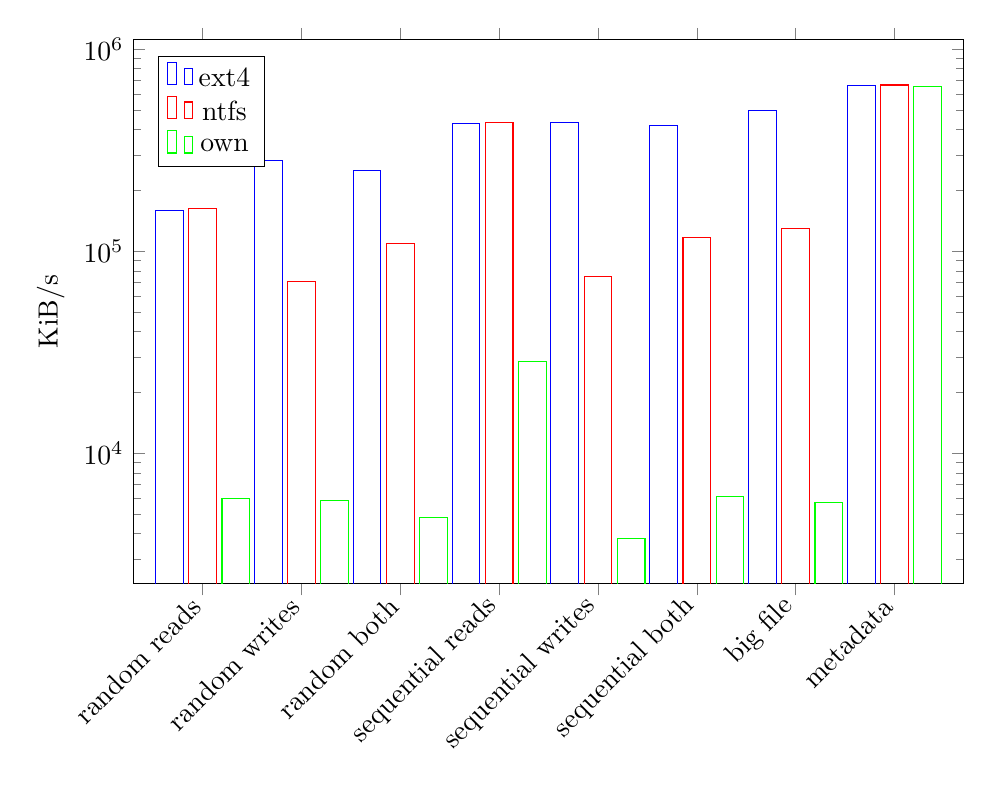
\begin{tikzpicture}
\begin{axis} [
    % TODO: add labels on data (useful)
    ybar, ymode = log,
    ylabel = {KiB/s},
    % nodes near coords,
    % nodes near coords align = {vertical},
    % enlargelimits=0.1,
    width=\textwidth, height = 0.7\textwidth,
    symbolic x coords = {
        random reads, random writes, random both,
        sequential reads, sequential writes, sequential both,
        big file, metadata
    },
    x tick label style = {rotate = 45, anchor = east},
    legend pos = {north west}
]

    % ext
    \addplot[
        draw=blue
    ] coordinates {
        (random reads, 159403) (random writes, 280917) (random both, 250539)
        (sequential reads, 430421) (sequential writes, 432469) (sequential both, 417792)
        (big file, 497323) (metadata, 663893)
    };

    % ntfs
    \addplot[
        draw=red
    ] coordinates {
        (random reads, 162133) (random writes, 70519) (random both, 109670)
        (sequential reads, 431445) (sequential writes, 74684) (sequential both, 116395)
        (big file, 128956) (metadata, 664576)
    };

    % own
    \addplot[
        draw=green
    ] coordinates {
        (random reads, 5963) (random writes, 5812) (random both, 4820)
        (sequential reads, 28331) (sequential writes, 3799) (sequential both, 6104)
        (big file, 5693) (metadata, 651947)
    };

    \legend{ext4, ntfs, own};

\end{axis}
\end{tikzpicture}

            \label{fig_benchmark}
        \end{figure}

        The ext4 and ntfs controls appear to behave as expected. Their
        performance is comparable although ntfs performs worse across the board
        as it is not natively implemented on Windows and the Linux driver has
        historically been lagging behind. Regardless, the ext4 results are a
        best case maximum whereas the ntfs ones are a more realistic
        representation of an imperfect filesystem implementation. The ntfs-3g
        driver is a reverse engineering effort of the proprietary ntfs
        filesystem and has been notorious for having a problematic
        implementation.

        The proposed filesystem performs an order of magnitude slower across
        the board. From the design stage (\ref{sec_design}) performance was
        expected to be worse due to the simplified design and out of kernel
        FUSE implementation. Random reads and writes are of comparable speed.
        This is not surprising, as the code paths they take are similar. Each
        access needs to have its destination resolved and then data written in
        the same way. Interestingly, however, sequential reads are about an
        order of magnitude higher than the overall perfomance of the
        filesystems and the corresponding sequential writes. This cannot be
        attributed to drive access assymetry, as the difference tends to be
        linear in SSDs \cite{servethehome_review}. Ext4 handles both workloads
        identially, supporting this idea. To confirm this, and investigate the
        cause, profiling analysys is performed in \ref{sec_perf}.

        The large file access is in line with the combined sequential test
        indicating that further increasing the work load does not reduce
        performance. Finally, the metadata benchmark is surprising as it is in
        line with ext4 and ntfs. This confirms the idea that for relatively
        small directories, a linear search does not make a big enough time
        contribution to outweighs other operations.

    \section{Profiling analysys}
        \label{sec_perf}

        To investigate the reasons for the performance the filesystem was
        profiled with perf \cite{perf}. Perf is powerful Linux tool (part of
        the kernel) for program profiling. It can produce performance
        statistics for hardware (cache hits, idle CPU cycles etc) and for
        sofware (call graphs, call frequency, work in each subroutine etc.).

        A profile was taken with \monospace{perf record -g <filesystem>}. For a
        workload, a full run of the benchmark was used \ref{sec_benchmark}.
        Then, the resulting 147Mb profile was manually analysed with
        \monospace{perf report -n --children} and \monospace{perf report -n
        --no-children}. The output of these two commands can be found in
        appendix \ref{app_perf}.

        Unsurpsiginly, most of the time is spent in the kernel (upwards of
        90\%). However, looking into which subroutine enters the kernel (with
        \monospace{--children}) has interesting results. The biggest time
        consumer is, as expected the file access subroutine
        (\monospace{do\_read\_write\_full()}). However, in it direct block
        read/write calls (with \monospace{read\_block()} and
        \monospace{write\_block()}) do not make up even a quarter of the time
        spent. Instead, an overwhelming majority of it is spent in btree
        accesses (\monospace{btree\_lookup64()} in this case) which indirectly
        call those subroutines. Inspecting the code provides two reasons.
        First, each block is located independently of all others and the quick
        access of sequential keys in the \bplustree (see \ref{sec_btree}) is
        not utilised. Additionally, large writes are handled like a sequence of
        small writes (with \monospace{do\_read\_write\_block()}). Even if
        sequences of blocks were to be accesses efficiently, this could not be
        observed by the read/write subroutines as they never receive them.
        Instead, they receive it split up into chunks. Another factor is that
        these inefficient accesses are not cached in any way to speed up
        subsequent similar accesses. Then the logarithmic benefit of the B-tree
        search is simply dwarfed by the sheer quanitfy which is performed. As a
        result, even large sequential workloads behave like numerous random
        ones and a lot of performance is left on the table.

        Knowing this, explaining the sequential read anomally is not hard. With
        this arrangement reading any file will always be faster than writing it
        due to a single factor - file expansion. By definition, when reading a
        file it cannot change its size. However, this does happen when writing
        it. Setting the file size in advance is not supported
        (\ref{sec_operations}) so the only place this can happen is on file
        write. Since all blocks get handled individually, each time the file is
        allocated the B-tree must be traveresed from the start. Then a
        potentially linear allocation must also happen. What is worse is that
        this happens on top of the traversal that has already been perfomerd to
        attempt to locate the block, resulting in an exponential time
        requirement. This stacks the penalty twice which reads simply do not
        do.

        From this analaysys arises a corollary: allocation cannot be fast. And
        in fact this is the reason why even the largest test is relatively
        small for today's standards. Since all accesses are split into blocks
        and treated individually, allocating a gigabyte of space with 4096 byte
        blocks requires an allocaiton for each or $2^{30} / 4096 \approx
        \numprint{262000}$ calls to the allocation subroutine. Since it the
        free list is also linear, after a period of use the search for free
        blocks start to dominate the required time.

        % Analyse the free list, maybe the i-list?
        % do a complexity analysys

        % Virtually all accesses in this filesystem require a file access,
        % becasue their metadata is stored in files (\ref{sec_files}). Since they
        % are also accessed with these subroutines, all workloads behave
        % identically.

        The overall poor performance cannot be attributed to a single factor,
        however, instead being a combination of smaller things. First, the
        impact of the individual treatment of blocks propagates throughout the
        filesystem, unituitively even in random accesses. This individuality
        only directly impacts sequentail access, as previously described.
        However, random accesses depend on lookups in the i-table, free list
        and directories which are themselves files. Accessing those is a
        sequential task but it performs in a random manner. So once again, the
        penalty stacks for an exponential decrease in performance, as we
        observe.


% actual percents. TODO: put in listing?
% -   93.79%     0.01%            36  filesystem   filesystem            [.] do_read_write_full
%    - 93.78% do_read_write_full
%       - 93.55% do_read_write_block
%          - 86.10% get_pblock_of_byte
%             + 86.10% btree_lookup64
%          + 6.44% file_add_space
%          + 0.61% __libc_pread


    \section{Failure simulation}

        To simulate failures we use a similar approach to the benchmark. Once
        again, we use fio. This time a 5 minute stress test is perfomerd. It
        has two jobs which run concurrently. The first one preforms the same
        1GB combined read and write load while the second one creates and
        removes 100 files repeatedly. While this test is running a script
        (\monospace{insert\_failures.py}) goes over the a drive in the array
        and flips a random number of bits on each block up to a maximum of 100
        in an infinite loop.

        As expected, the whole test runs without any user visible errors. The
        filesystem detects and corrects all corrupt blocks and returns correct
        data stored on the redundant drives.

        % TODO: add a figure with the debug output that the error was detected and fixed

    \section{Design of the redundancy}

        As shown experimentally, the integrity guarantee works. Theoretically,
        best case security of the 256 bit hashes are $2^{128}$ bits.
        Theoretical attacks on reduced versions of the function put this at
        $2^{126}$ \cite{sha2_security} \cite{sha2_analysis}. At this time
        SHA256 does not have any known collisions. So for the purposes of this
        project we consider it as secure with $2^{126}$ bits of security (we
        select the lower bound for safety). Thus the probability that a faulty
        sector results in a hash collision will be at most $2^{-126}$. It is
        important to note that errors are not entirely arbitrary but rather
        follow some patterns (\ref{sec_reliability}) and are likely to have
        very few bits changed. Therefore for normal wear and tear the
        probability of a collision is likely to be much lower due to the
        avalanching effect of the funciton, however, this has not been
        theoretically verified and is not be relied upon.

        Unlike ZFS \ref{sec_ZFS}, this filesystem does not chain checksums.
        Therefore it is possible two blocks (one data and one hash) to corrupt
        in such a way that the checksum is still valid. ZFS's chaining of
        hashes mitigates against this. However, the chance of this happening is
        astronomically low. As the errors are independent on SSDs
        \ref{sec_reliability} the likelyhood of that happening with SHA256
        will be $2^{252}$. This is a valid issue to have with short (eg. CRC)
        checksums however with our long hashes this issue can be safely
        ignored. Regardless, the alternation of data and checksum accesses
        (\ref{sec_data_integrity}) between the two drives makes this
        impossible.

        In the event of malicious loads, like a rowhammer derivative attack
        \cite{ssd_rowhammer}, the security is likely to be lower as the
        attacker can craft the payload more carefully. However, the
        checksumming of the data provide a barrier to pulling off such an
        attack despite any ability for controlling failures the attacker might
        have. In effect this acts like stack canaries \cite{canary} as it is
        an extra, unknown, value that is assumed to be difficult to acces and
        predict by the attacker. We can conclude that since the checksum is at
        least slightly separate its modificaiton will be extremely difficult
        and if it is possible, the security of the hash function can be relied
        upon.

    % \section{Technical evaluation?}
    % TODO: Appropriate technical and/or user evaluation.
    % Results clearly related to motivation/goals as appropriate

    % \section{Implementation}

    %     As noted in the performance analysys \ref{sec_perf}, this filesystem's
    %     performance is not on par with what is available. Separately, it
    %     experiences occasional crashes and instability, independently of the
    %     reliability mechanisms. As a proof of concept, this is deemed to be
    %     acceptable, however it should be noted that further work is required to
    %     develop this filesystem into a usable product.
